\documentclass[12pt]{article}
\usepackage{fullpage,enumitem,amsmath,amssymb,graphicx, multicol, algorithm2e, algorithmicx}

\begin{document}

\begin{center}
{\Large Adapting Fukushima's Neocognitron for Optical Character Recognition of English Handwritten Characters}

\begin{tabular}{rl}
Andrew Giel & Computer Science 2015
\end{tabular}
\end{center}

\textit{With his seminal paper in 1988, Fukushima presented a hierarchical network capable of complex visual pattern recognition named the Neocognitron which he applied to the task of handwritten numeral recognition. This paper presents a modern-day implementation of the Neocognitron theoretically capable of invariant recognition of English handwritten characters.}

\section{Introduction}

In 1980 Kunikho Fukushima and the NHK Science and Techincal Laboratories presented the idea of the Neocognitron, a feed-forward neural network able to visually recognize handwritten numerals. In 1988, they followed up on this inventive theoretical paper by publishing a paper describing an implemented and functional instance of the Neocognitron. This network was biologically inspired by the findings of Hubel and Weisel, who found neurons in the primary visual cortex of cats that had high firing rates in response to oriented lines of different angles. Hubel and Weisel also found that paired with these orientation-specific cells, which they called simple cells, were cells with a higher degree of spatial invariance (larger receptive fields) in their responses and were possibly capable of motion detection. Fukushima and his team, employing these monumental findings in the field of neurophysiology, modeled the Neocognitron in a similar fashion, alternating between layers of Simple cells, $S$ layers, and layers of Complex cells, $C$ layers. With these alternating $S$ and $C$ layers capable of both selectivity and invariance, Fukushima trained the Neocognitron to recognize progressively more complex patterns, creating a feed-forward hierarchy with the last layer of $C$ cells being the gnostic or so called $grandmother$ cells of the system. Fukushima's Neocognitron was a groundbreaking achievement, changing the field indefinitely with his use of the biologically inspired alternation of selectivity and invariance. The Neocognitron made it clear to the academic community that convolutional neural networks were not only biolgically feasable, but also robust and accurate. 

\section{Modern Optical Character Recognition}
Since the days of Fukushima, advances in computing have allowed for great progress in the task of Optical Character Recognition (OCR), yet Fukushima's original solution to the problem of invariance yet selectivity via alternating cell layers remains to this day the basis for this technological progress.

One of the most prominent academics in the field of visual object recognition, Yann LeCun, has published many papers which use the concepts presented by Fukushima in the Neocognitron paper. In particular, LeCun along with AT\&T Bell Labs published a paper in 1989 entitled ``Backpropagation Applied to Handwritten Zip Code Recognition'' in which a network capable of recognizing the zip codes on postage is described. The network is trained via the back-propagation algorithm made famous by Rumelhardt, and consists of 5 layers; the input layer, three hidden layers denoted $H_1$, $H_2$, and $H_3$ respectively, and the output layer. Referencing Fukushima's 1980 paper as ``classicsal work in visual pattern recognition'' LeCun notes the advantages of extracting local features and combining them in a hierarchical fashion- unable to identify the exact location of features yet still knowing the approximate location. This of course references the simple and complex cells of Hubel and Weisel made known to the computing community by Fukushima. LeCun's network, like the Neocognitron, uses planes within layers as feature maps and each plane shares the weights of its connections via a single parameter (``weight sharing''). Unlike Fukushima, LeCun trains his network by showing example images and then back-propagating, removing the expensive necessity to create templates. The weights are updated using stochastic gradient descent. LeCun's network uses the $\tanh$ function for its non-linearity in the equivalent of the complex cells, and the cost function was mean squared error.  

The experimental results of this paper are quite remarkable with low error rates (\%5.0) on a large test set with inputs that vary significantly between cases. The network displays the type of selectivity and invariance so celebrated by Fukushima in the Neocognitron, applied to a real world task. A similar network is employed today by the US Postal Service. 

\section{Goal of Computational Testing}
This paper is inspired by two concepts presented in Fukushima's 1988 publication. 

The first conceptual motivation comes from Fukushima discussing the capabilities of the Neocognitron. Fukushima claims, ``Since the Neocognitron can learn, it can be trained to recognize not only Arabic numerals, but also other sets of patterns, like the letters of the alphabet, geometrical shapes, or others. Hence, it is possible to design a Neocognitron as a univeral pattern-recognizer, which can be used, after training, for an individual purpose.'' This paper tests the robustness of these claims by applying the Neocognitron architecture to handwritten letters of the alphabet. By creating a network with similar properties and parameters to the originally published network, this paper tests to what degree the Neocognitron is ``universal'' and how successful it can be in a task with significantly larger output space.

Another claim made by Fukushima also inspired this paper. Fukushima goes in depth regarding the distinction between learning with and without a ``teacher''. In order for the network to learn, or in other words to train the network, a series of training templates are presented to the layers, each cell plane of the layer receiving a different template corresponding to a different feature which that plane learns to identify. As mentioned earlier, these features, and subsequently the templates, become progressively more complex until they are full representations of the pattern intended to be recognized. The ``teacher'' comes in to play after the cell plane has been presented with the template, when the network must adjust its parameters to learn the template so that the plane becomes selective to the feature. This is done for the whole plane on behalf of one cell, the seed-cell. The entire plane's parameters are changed based on a single cell's response to the stimulus. In the 1988 paper, Fukushima used learning with a teacher, by selecting the seed cell for each template manually. Yet learning without this teacher is also possible according to Fukushima, by selecting the cell with the maximum output as the seed cell. This paper's implementation focuses on learning without a teacher, further differentiating itself from the original publication and testing the limits to which Fukushima's claims are true for different tasks. 

\section{Implementation}
This paper's implementation was adapted from a public GitHub repository from GitHub user nicholasjconn. It consisted of 7 layers, $S_0$, $S_1$, $C_1$, $S_2$, $C_2$, $S_3$, and $C_3$. This is effectively 3 layers of feature extraction and pooling, one less than that of Fukushima despite a task with a larger output space (10 vs 26). The reason for this discrepancy is the cost of making training feature templates, which are very expensive and outline one of the largest downfalls of this network. 
\begin{center}
  \begin{tabular}{| c | c | c |}
  \hline 
  Layer & Plane Size & \# Planes \\ \hline
  $S_1$ & 19$\times$19 & 12 \\ \hline
  $C_1$ & 21$\times$21 & 12 \\ \hline
  $S_2$ & 21$\times$21 & 28 \\ \hline
  $C_2$ & 13$\times$13 & 28 \\ \hline
  $S_3$ & 13$\times$13 & 26 \\ \hline
  $C_3$ & 1$\times$1 & 26 \\
  \hline
  \end{tabular}
\end{center}

Learning without a teacher was implemented in this network. For each layer $S_k$, the training inputs are fed to the prior layers $S_1 \to S_{k-1}$, and then exposed to $S_k$. For each plane $s_i \in S_k$ a seed cell $\hat{n} \in s_i$ is designated by determining the maximum output cell $\hat{n} = \max_{n \in s_i} u_{S_k}(n, i)$ where $u_{S_k}(n, i)$ indicates the response of the cell $n$ in the plane $i$ of layer $S_k$. From here, the variable learnt connectivity strengths $a$ and $b$ can be altered according to equations 5 and 6 of Fukushima 1988. 

Figures (1) (2) and (3) show examples of training templates for $S_1$, $S_2$, and $S_3$ respectively. 

\begin{figure}[ht!]
\centering
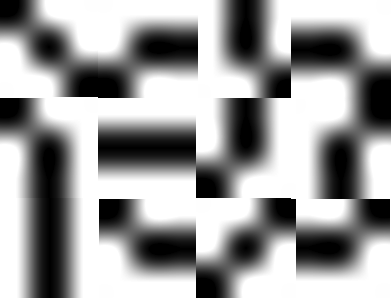
\includegraphics[width=90mm]{firstLayer.png}
\caption{Example Templates for $S_1$}
%\label{overflow}
\end{figure}

\begin{figure}[ht!]
\centering
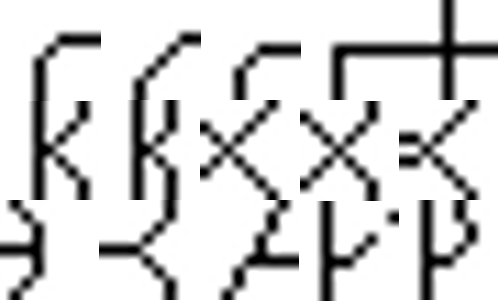
\includegraphics[width=90mm]{secondLayer.png}
\caption{Example Templates for $S_2$}
%\label{overflow}
\end{figure}

\begin{figure}[ht!]
\centering
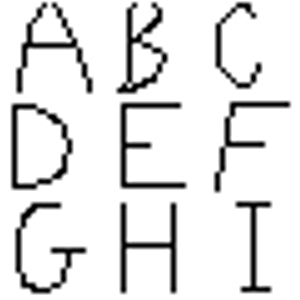
\includegraphics[width=90mm]{thirdLayer.png}
\caption{Example Templates for $S_3$}
%\label{overflow}
\end{figure}

\section{Results}
Unfortunately, at time of writing, this implementation is non-functional. For any given test input, the output of $C_3$, the so-called gnostic cells, are similar across all 26 planes of the layer. Their outputs are asymptotically close to 1, the max output possible for a complex cell. As such, when the network attempts to infer the output of the system by finding the plane with the highest output in $C_3$, it is essentially randomly picking a plane and therefore an output. As would be expected, this leads to an error rate of about 95\%, or 1 - (1/26). 

Attempts to debug this issue have proven unfruitful. 

This author had a few suspicions regarding numpy (as this network was written in python) encoding of images being the culprit, yet ensuring the images were expressed as binary bitmaps of pixels did not help. Addtionally, earlier iterations of the implementation suffered from overflow/underflow issues that possibly could have compromised the network, yet simple measures were taken to ensure this did not happen and unfortunately did not improve effectiveness.

This author's main approach to debug was to visualize the acivations of the planes within $C_1$ and $C_2$ in hopes they would reveal the behavior in play. Note $C_1$ and $C_2$ should, in a functional network, express the local pattern matches or features recognized. Unfortunately, the outputs of $C_1$ and $C_2$ do not look especially suspicious and seem to, in some capacity, be representing the feaures they should be. This, paired with parameter adjustment, seems to be the best course of action for future investigation into why the current system does not function as expected. 

\section{References}
Fukushima, 1980. \\
$http://www.cs.princeton.edu/courses/archive/spr08/cos598B/Readings/Fukushima1980.pdf$ \\\\
Fukushima, 1988. \\
$http://hebb.mit.edu/courses/9.641/2006/readings/Fukushima88.pdf$ \\\\
Hubel and Weisel, 1962. \\
$http://www.ncbi.nlm.nih.gov/pmc/articles/PMC1359523/pdf/jphysiol01247-0121.pdf$ \\\\
LeCun, 1989. \\
$https://www.ics.uci.edu/~welling/teaching/273ASpring09/lecun-89e.pdf$ \\\\
Rumelhardt, 1986. \\
$http://www.nature.com/nature/journal/v323/n6088/pdf/323533a0.pdf$ \\\\

\end{document}
